\documentclass{beamer}
%
% Choose how your presentation looks.
%
% For more themes, color themes and font themes, see:
% http://deic.uab.es/~iblanes/beamer_gallery/index_by_theme.html
%

% Theme License: https://creativecommons.org/licenses/by/4.0/

\mode<presentation>
{
  \usetheme{metropolis}   % https://github.com/matze/mtheme
  \usecolortheme{default} % or try albatross, beaver, crane, ...
  \usefonttheme{default}  % or try serif, structurebold, ...
  \setbeamertemplate{navigation symbols}{}
  %% \setbeamertemplate{caption}[numbered]
  \setbeamertemplate{caption}{\raggedright\insertcaption\par}
}

\usepackage[english]{babel}
\usepackage[utf8x]{inputenc}

\title{An Introduction to \LaTeX}
\author{Jake Vossen}
\institute{Colorado School of Mines - acm-w}
\date{2020-02-26}

\begin{document}
\begin{frame}{Something to consider...}
    \begin{figure}
    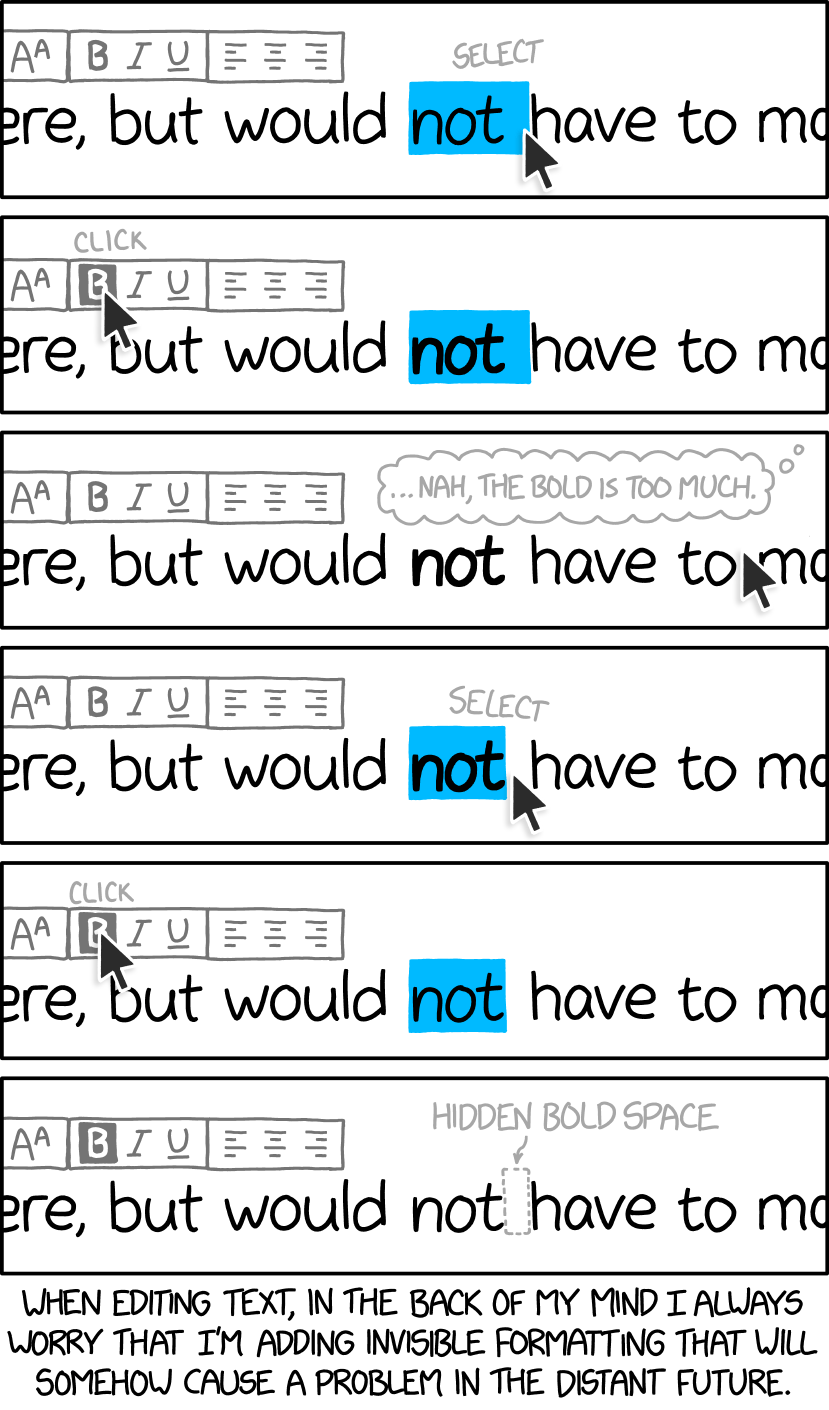
\includegraphics[scale=.13]{invisible_formatting_2x.png}
    \caption{https://xkcd.com/2109/}
  \end{figure}
\end{frame}
\begin{frame}
  \titlepage
\end{frame}

% Uncomment these lines for an automatically generated outline.
%\begin{frame}{Outline}
%  \tableofcontents
%\end{frame}

\section{The Why}

\begin{frame}{First Slide}


\vskip 1cm

\end{frame}

\end{document}
